\documentclass[11pt,a4paper]{article}
\usepackage[margin=2.3cm]{geometry}
\usepackage[T1]{fontenc}
\usepackage{textcomp}
\input{glyphtounicode}
\pdfgentounicode=1
\usepackage{lmodern}
\usepackage{xcolor}
\usepackage{listings}
\usepackage{tcolorbox}
\usepackage{booktabs}
\usepackage{array}
\usepackage{tikz}
\usepackage{hyperref}
\hypersetup{colorlinks=true, linkcolor=blue!50!black, citecolor=green!40!black}

\definecolor{codebg}{RGB}{248,248,245}
\lstset{
  language=C, basicstyle=\ttfamily\footnotesize, backgroundcolor=\color{codebg},
  keywordstyle=\color{blue!60!black}\bfseries, commentstyle=\color{green!45!black}\itshape,
  stringstyle=\color{red!60!black}, numbers=none, upquote=true,
  frame=single, rulecolor=\color{gray!40}, breaklines=true, columns=fullflexible,
  keepspaces=true, showstringspaces=false
}
\lstdefinestyle{sh}{language=bash, backgroundcolor=\color{black!5}}

\newtcolorbox{keyidea}{colback=blue!4, colframe=blue!45!black, title=Key ideas, fonttitle=\bfseries\small}
\newtcolorbox{experiment}{colback=orange!5, colframe=orange!70!black, title=Experiment, fonttitle=\bfseries\small}

\title{\textbf{OpenMP --- Lesson 6}\\[4pt]\large Coordinating the team: \texttt{barrier}, \texttt{single} and \texttt{sections}}
\author{Gustavo Lozano}
\date{November 2026}

\begin{document}
\maketitle

\noindent\textit{\small Source: Chapman, Jost \& van der Pas~\cite{chapman}, Ch.~4
``OpenMP Language Features'' (the \texttt{single} and \texttt{sections} work-sharing
constructs and the \texttt{barrier} synchronization construct).}

\section{The idea}
Lesson~4 split a \emph{loop} among threads. But a parallel region often contains other
kinds of work:
\begin{itemize}
  \item a step that must be done \textbf{once}, not by every thread (read input, fill an
        array, print a result) $\to$ \texttt{single};
  \item a few \textbf{different}, independent tasks that can run at the same time
        $\to$ \texttt{sections};
  \item a point that \textbf{all} threads must reach before any continues, because the
        next phase needs the results of the previous one $\to$ \texttt{barrier}.
\end{itemize}

\begin{center}
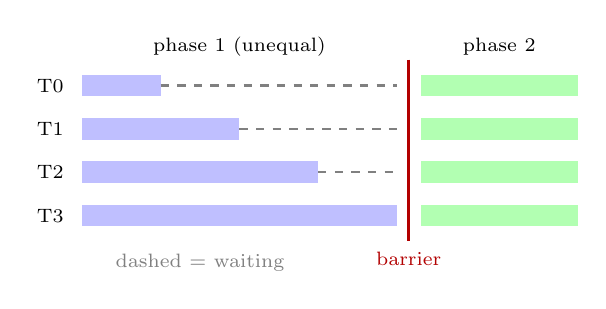
\begin{tikzpicture}[thick, x=1cm, y=0.55cm]
  \foreach \t/\len in {0/1,1/2,2/3,3/4} {
    \node[font=\scriptsize, anchor=east] at (-0.1,-\t) {T\t};
    \fill[blue!25] (0,-\t-0.25) rectangle (\len,-\t+0.25);
    \draw[dashed, gray] (\len,-\t) -- (4,-\t);
    \fill[green!30] (4.3,-\t-0.25) rectangle (6.3,-\t+0.25);
  }
  \draw[red!70!black, very thick] (4.15,0.6) -- (4.15,-3.6) node[below, font=\scriptsize] {barrier};
  \node[font=\scriptsize] at (2,0.9) {phase 1 (unequal)};
  \node[font=\scriptsize] at (5.3,0.9) {phase 2};
  \node[font=\scriptsize, gray] at (1.5,-4.1) {dashed = waiting};
\end{tikzpicture}
\end{center}

\section{The three constructs}
\begin{center}
\small
\begin{tabular}{@{}>{\raggedright\arraybackslash}p{3.6cm}>{\raggedright\arraybackslash}p{7.6cm}>{\raggedright\arraybackslash}p{4.0cm}@{}}
\toprule
Construct & What it does & Barrier at the end? \\ \midrule
\texttt{\#pragma omp barrier} & every thread waits here until all threads of the team
  arrive & it \emph{is} a barrier \\
\texttt{\#pragma omp single} & the block is run by exactly \textbf{one} thread (any one);
  the others skip it & yes (removable with \texttt{nowait}) \\
\texttt{\#pragma omp sections} with several \texttt{\#pragma omp section} & each
  \texttt{section} is a different block, run exactly once by some thread of the team
  & yes (removable with \texttt{nowait}) \\
\bottomrule
\end{tabular}
\end{center}
\texttt{single} and \texttt{sections} are \textbf{work-sharing} constructs, like
\texttt{for}: they divide work among the threads that already exist, and do not create
new ones. They must appear inside a \texttt{parallel} region.

\section{The code}
Part 1 gives each thread an unequal phase~1 (thread $k$ sleeps $0.1k$ seconds), then a
barrier, then phase~2. Part 2 uses \texttt{single} to fill an array once, two
\texttt{sections} to compute its sum and its maximum, and a second \texttt{single} to
print the result.
\lstinputlisting[title=\texttt{single\_sections.c}]{single_sections.c}

\begin{lstlisting}[style=sh]
gcc -Wall -fopenmp -o single_sections single_sections.c
OMP_NUM_THREADS=4 ./single_sections
\end{lstlisting}
Typical output (thread numbers and order will differ):
\begin{lstlisting}[style=sh]
--- Part 1: barrier ---
  thread 0 finished phase 1
  thread 1 finished phase 1
  thread 2 finished phase 1
  thread 3 finished phase 1
  thread 3 started  phase 2
  thread 1 started  phase 2
  thread 0 started  phase 2
  thread 2 started  phase 2
--- Part 2: single and sections ---
  thread 3 fills the array (single)
  thread 2 computed sum (section 1)
  thread 2 computed max (section 2)
  thread 3 prints: sum = 4986, max = 100 (single)
\end{lstlisting}

\begin{keyidea}
\begin{itemize}
  \item With the barrier, \emph{all} ``finished phase 1'' lines come before
        \emph{any} ``started phase 2'' line, even though thread 0 finished 0.3\,s
        before thread 3.
  \item \texttt{single}: the array is filled once. Its implicit barrier is what
        guarantees that no thread starts reading \texttt{a[]} before it is full.
  \item \texttt{sections}: each section runs exactly once, but you do not choose the
        thread. Short sections are often both taken by the same thread, as in the
        output above. Sections guarantee \emph{once}, not \emph{in parallel}.
  \item No race on \texttt{sum} or \texttt{max}: each is written by only one section,
        and the final \texttt{single} reads them after the barrier of \texttt{sections}.
\end{itemize}
\end{keyidea}

\section{The experiment}
\begin{experiment}
\textbf{Question:} what does the barrier actually guarantee?
\begin{enumerate}
  \item Run the program as it is, several times, and look at Part~1:
\begin{lstlisting}[style=sh]
for r in 1 2 3; do OMP_NUM_THREADS=4 ./single_sections | head -9; echo; done
\end{lstlisting}
  \item Comment out the barrier in Part~1, recompile, and run again:
\begin{lstlisting}
        /* #pragma omp barrier */
\end{lstlisting}
  \item In the same runs, note which thread executes each \texttt{single} and each
        \texttt{section} in Part~2.
\end{enumerate}
\textbf{What to observe and answer.}
\begin{enumerate}
  \item Without the barrier, how are the phase~1 and phase~2 lines ordered now? Why?
  \item Suppose phase~2 read a value that \emph{every} thread wrote in phase~1. What would
        go wrong without the barrier?
  \item Is the thread that runs a \texttt{single} always the same? Is it always thread 0?
\end{enumerate}
\end{experiment}

\paragraph{Answers (read after trying).}
(1)~Each thread starts phase~2 right after its own phase~1, so the lines appear in pairs
(thread 0 finishes and starts, then thread 1, \ldots). Nothing makes a thread wait for
the others.
(2)~A fast thread would start phase~2 while slow threads are still writing their phase~1
values, and would read incomplete data. That is a race between phases, and it is exactly
what a barrier prevents.
(3)~No. The standard leaves the choice to the implementation; in practice it is usually
the first thread to arrive, which changes from run to run. If the work must be done by the master thread, OpenMP has a separate
construct, \texttt{master} (renamed \texttt{masked} in recent versions), which, unlike
\texttt{single}, has \emph{no} implicit barrier.

\paragraph{Next lesson.} Tasks: the \texttt{task} and \texttt{taskwait} constructs, for
work that is not a loop and whose size is not known in advance (van der Pas
et al.~\cite{vdp}, chapter on tasking).

\begin{thebibliography}{9}
\bibitem{chapman} B.~Chapman, G.~Jost, and R.~van der Pas. \emph{Using OpenMP: Portable
  Shared Memory Parallel Programming}. MIT Press, Cambridge, MA, 2007.
\bibitem{vdp} R.~van der Pas, E.~Stotzer, and C.~Terboven. \emph{Using OpenMP --- The Next
  Step: Affinity, Accelerators, Tasking, and SIMD}. MIT Press, Cambridge, MA, 2017.
\end{thebibliography}
\end{document}
